\documentclass[11pt]{article}
\usepackage[margin=1in]{geometry}
\usepackage{amsmath,amssymb,amsthm}
\usepackage{graphicx,booktabs,longtable,hyperref,xcolor}
\usepackage[numbers]{natbib}
\hypersetup{colorlinks=true,linkcolor=blue!50!black,citecolor=blue!50!black,urlcolor=blue!50!black}
\newcommand{\todo}[1]{\textcolor{red}{[TODO: #1]}}
\newtheorem{theorem}{Theorem}

\title{Twelve Unit Cubes in a Cube of Side 2.9315,\\ Found by Hardening Balls into Cubes}
\author{Yohei Nakajima\thanks{\texttt{yohei@untapped.vc}. Experiments, code and verification were developed with the assistance of Claude (Anthropic); see the acknowledgements.}}
\date{8 October 2026}

\begin{document}
\maketitle

\begin{abstract}
We give a packing of 12 unit cubes in a cube of side $2.9315185$, with every pair and every wall at least $10^{-6}$ apart, improving the previous best known side $2.9327717687$ (H.~Lin, July 2026 \cite{hyra}). The packing was found by a soft-to-rigid homotopy: unit-diameter balls are compressed in a shrinking box and then deformed through rounded cubes into rigid unit cubes while inward pressure on the box continues. The final configuration is tightened with a constrained solver that keeps every corner inside the box and a separating plane between every nearby pair, and validated by an exact rational certificate. On unit squares in a square, the same method recovers the best known packings for $n=11$ (now proved optimal), $17$, $18$, $19$, $26$ and $27$, and outperforms a rigid-start control on the same seeds. We report where the method fails ($n=28,29$ squares; $n=10,11$ cubes so far), an ablation showing that an oriented intermediate shape does not help, and code to reproduce every result.
\end{abstract}

\section{Introduction}
Let $s_d(n)$ be the side of the smallest $d$-dimensional cube that contains $n$ non-overlapping unit cubes, free to rotate. For squares ($d=2$) the problem has a long record history \cite{erdosgraham,stromquist,friedmansurvey,squaresproject}; the smallest unsettled case, $n=11$, was recently closed \cite{squaresproject}. For cubes ($d=3$) far fewer results exist. Friedman's catalogue \cite{friedmancubes} lists non-trivial packings for $n=9$--$14$ and $28$--$33$; the entries for $n=11$ and $12$ were improved in 2026 (T.~Berthold et al.\ in March for $n=11$; H.~Lin in July for $n=11$ and $12$, with coordinates published in \cite{hyra}), and for every other $n<34$ the trivial packing is the best known.

\paragraph{Contribution.}
\begin{enumerate}
\item A packing of 12 unit cubes in a cube of side $2.9315185094797$ with every pair and every wall separated by at least $10^{-6}$ (\S\ref{sec:record}), $0.0012533$ below the previous record $2.9327717687048653$. It is certified in exact rational arithmetic.
\item A simple search method, soft-to-rigid homotopy with inward pressure (\S\ref{sec:method}), and an exact tightening step that turns its output into a locally optimal packing to $10^{-12}$.
\item An empirical record of what the method does and does not reach: in 2D it recovers six published records from random starts and beats a rigid-start control; it fails on $n=28,29$ squares; an oriented intermediate shape does not raise its hit rate (\S\ref{sec:squares}, \S\ref{sec:ablations}).
\end{enumerate}
This is a search result, not an optimality proof.

\paragraph{Related methods.} Gensane and Ryckelynck's perturbation--compression algorithm found dense square packings, including $n=11$, from random starts \cite{gensane}. Recent square records ($n=28$, $29$, $39$, $41$, $50$, $51$, $55$) come from rigid simulated annealing and exact refinement \cite{squaresproject}. Our method differs in starting from balls and changing the shapes, not just their positions, during the search.

\section{Method}\label{sec:method}
\paragraph{Shape family.} A \emph{rounded cube} of softness $r\in[0,\tfrac12]$ is a cube of half-side $\tfrac12-r$ dilated by a ball of radius $r$ (the Minkowski sum). At $r=\tfrac12$ it is a unit-diameter ball, at $r=0$ a unit cube, and every member lies inside the unit cube with the same centre and orientation. Hardening ($r\downarrow 0$) therefore only grows the shapes, and the container must expand to accommodate them. The square version uses rounded squares.

\paragraph{Energy and pressure.} For centres $c_i$, orientations $q_i$ (quaternions in 3D, angles in 2D) and container side $L$,
\[
E=\sum_{i<j}\big(2r-\operatorname{sd}(i,j)\big)_+^2+\sum_i\sum_{\text{walls}}(\text{violation})_+^2+\mu L,
\]
where $\operatorname{sd}(i,j)$ is the signed distance between the cores (cube of half-side $\tfrac12-r$): exact Euclidean distance when separated (vertex--face and edge--edge features), and minus the separating-axis penetration depth when overlapping (15 axes for cubes \cite{gottschalk}). The term $\mu L$ is inward pressure; the box resizes symmetrically so all walls push. Positions, orientations and $L$ follow momentum gradient descent with analytic gradients (checked against finite differences on $72{,}000$ random cube-pair gradient components and $120{,}000$ square-pair components).

\paragraph{Schedule.} Compress balls under pressure $3\mu$ (5{,}000 steps); morph $r:\tfrac12\to0$ linearly at pressure $\mu=0.02$ (45{,}000 steps); settle rigid cubes while $\mu$ decays to $2\cdot10^{-6}$ (3{,}000 steps). Optional \emph{annealing} adds Gaussian kicks to positions and angles that decay to zero during compression and morphing. The \emph{rigid control} runs the identical schedule with $r=0$ throughout.

\paragraph{Legalization.} Penalty pressure tolerates small overlaps. Each run is legalized by scaling centres apart about their mean (bisection to the smallest factor at which no pair overlaps by more than $10^{-12}$ under the separating-axis test) and measuring the tight bounding cube. All sides reported below are legal packings.

\paragraph{Exact tightening.} Runs within a threshold of the catalogue are passed to a constrained solver: minimize $L$ over centres, rotations and per-pair separating planes $u_{ij}\cdot p=c_{ij}$, subject to every corner of every cube lying in $[0,L]^3$ and the corners of $i$ and $j$ lying on opposite sides of their plane. We use SLSQP \cite{kraft} in outer iterations with a trust region, rebuilding the pair list and re-basing rotations each iteration, and accept a step only if the independently legalized side decreases. From near-miss runs the solver converges to Trump's $s_2(11)$ \cite{trump} and Bidwell's $s_2(17)$ \cite{friedmansurvey} to $10^{-12}$, and from a perturbed copy to Friedman's $s_3(9)=2+1/\sqrt2$.

\paragraph{Exact certificate.} For a reported 3D packing we expand centres by a factor $1+10^{-6}$ about their mean and inflate each half-side to $\tfrac12(1+10^{-12})$, which covers floating-point non-orthogonality of the axes. We convert every coordinate to an exact rational, compute all corners exactly, and check (i) every corner lies in $[0,S]^3$ for a rational $S$ and (ii) every pair is strictly separated by an explicit rational plane. A linear program proposes each plane; the check itself uses only exact arithmetic.

\section{Twelve cubes}\label{sec:record}
\begin{theorem}
Twelve unit cubes fit in a cube of side $2.9315185094797$ with pairwise and wall clearance at least $10^{-6}$. Hence $s_3(12)\le 2.9315185094797<2.9327717687048653$.
\end{theorem}
\noindent\emph{Certificate.} The claim file (\texttt{claims/cubincub\_n12/cubincub\_n12.json}, Table~\ref{tab:coords}) lists one pose $[x,y,z,q_w,q_x,q_y,q_z]$ per cube, the format of the previous record file \cite{hyra}. It was obtained from the tightened packing (side $2.931514577965$, with touching contacts) by spreading centres by a factor $1+1.0\cdot10^{-6}$ until every pair is separated by $10^{-6}$, adding a $10^{-6}$ wall gap and rounding the side up. Two checks pass. (i) A floating-point 15-axis separating-axis test (\texttt{verify.py}, 30 lines): minimum wall gap $1.000000000\cdot10^{-6}$, minimum pair gap $1.000000001\cdot10^{-6}$. (ii) An exact check (\texttt{certify\_exact.py}): every number is converted to a rational, rotations are the exactly orthogonal $H(q)/|q|^2$, every corner lies in $[0,s]^3$ and every pair is strictly separated by an explicit rational plane.

Four cubes are exactly axis-aligned, two are tilted by less than $1^\circ$, and six are tilted by $9^\circ$ or more (Figure~\ref{fig:n12}). Several quaternions have repeated components (e.g.\ cube 1: $(0.58389,-0.58389,-0.39884,-0.39884)$), suggesting a closed form that we have not derived. We have not derived it.

\paragraph{How it was found.} Seed 52 of the first 64 ball$\to$cube starts with annealing ended at legalized side $2.931821$; exact tightening lowered it to $2.931514577965$. A second start (seed 83) ended at $2.931910$ and tightens to $2.931619541$: a distinct local optimum, also below the catalogue. Two of 192 starts land below $2.93277$. The rigid control's best of 32 starts is $2.99257$.

\begin{figure}[t]\centering
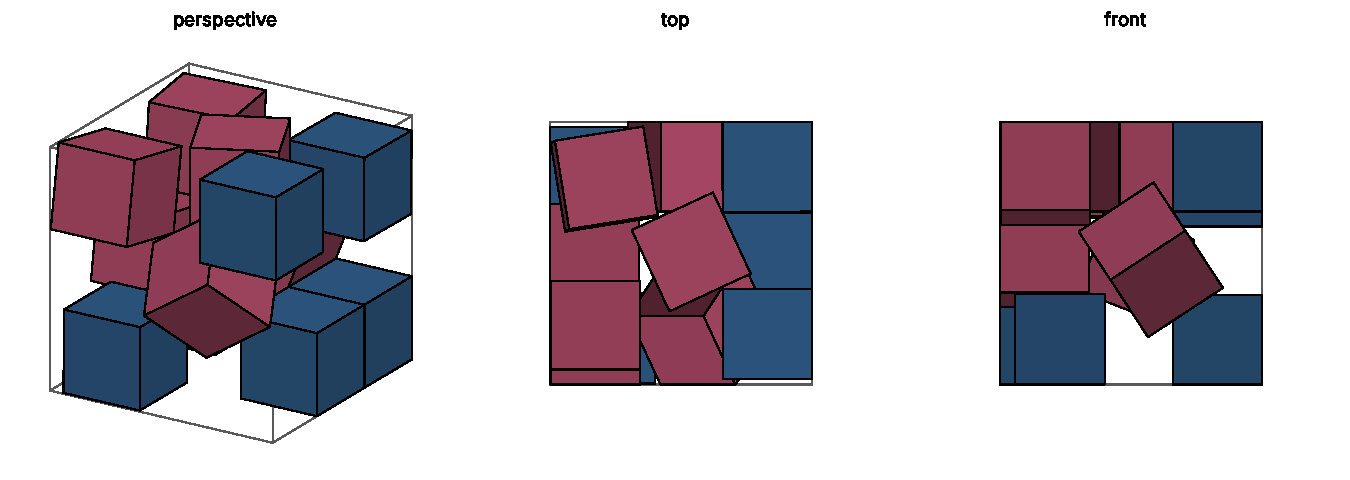
\includegraphics[width=\linewidth]{figures/n12_views.pdf}
\caption{Twelve unit cubes in a cube of side $2.931515$. Blue: tilt below $1.5^\circ$; red: tilted.}\label{fig:n12}
\end{figure}

\paragraph{Other cube counts.} Table~\ref{tab:cubes} summarizes the first 3D screen. The method matches Friedman's $n=9$ packing often, settles in worse arrangements at $n=10$ and $11$, and is the only setup that comes near the catalogue at $n=12$.
\begin{table}[h]\centering\small
\begin{tabular}{lrrrrr}\toprule
$n$ & catalogue & starts (ball / rigid) & best ball$\to$cube & best rigid & matches (ball / rigid)\\\midrule
9 & $2.70711$ & 64 / 32 & $2.707107$ & $2.707107$ & 16 / 5\\
10 & $2.70711$ & 64 / 32 & $2.767767$ & $2.894428$ & 0 / 0\\
11 & $2.88295$ & 64 / 32 & $2.894427$ & $2.918992$ & 0 / 0\\
12 & $2.93277$ & 192 / 32 & $\mathbf{2.931515}$ & $2.992573$ & --- \\
13 & $2.956$ & 48 / --- & $2.997184$ & --- & 0 / --- \\
14 & $2.98995$ & 42 / --- & $3.000000$ & --- & 0 / --- \\\bottomrule
\end{tabular}
\caption{First 3D screen (annealed ball$\to$cube vs.\ rigid control, $53{,}000$ steps per start; best after exact tightening). The best $n=10$ run is within $2\cdot10^{-7}$ of $1+5\sqrt2/4$; the tightened best $n=11$ run equals $2+2/\sqrt5\approx2.894427$ to $10^{-9}$, below the March 2026 value but above Lin's $2.8829529$.}\label{tab:cubes}
\end{table}

\section{Validation on squares}\label{sec:squares}
We developed the method on unit squares, where records are dense and recently audited \cite{squaresproject,friedmansurvey}.

\paragraph{$n=11$.} With annealing and the long schedule, 6 of 160 random starts reach Trump's packing (tilt $40.18^\circ$); 0 of 120 rigid-control starts do (best $3.8877$, median $4.000$). Trump's packing has since been proved optimal \cite{squaresproject}, so this is a sanity check.

\paragraph{$n=2$--$30$ at a fixed schedule.} Among cases whose best known packing has tilted squares, the method matches $n=5,10,11$ and none from $17$ upward at the standard step budget; the rigid control matches $5$ and $10$. Grid cases split by slack: when the grid has empty cells ($n=6,7,12,13,20,21$) rigid starts fall into it more often (46--100\% vs.\ 2--19\%), while for full or nearly full grids ($n=9,15,16,22$--$25,30$) rigid starts jam at tilts they cannot rotate out of (e.g.\ $n=25$: rigid 0/24, balls 7/48).

\paragraph{Old records recovered with more steps and exact tightening.}
\begin{table}[h]\centering\small
\begin{tabular}{llrl}\toprule
$n$ & best known (finder) & recovered to & hit rate\\\midrule
17 & $4.675530$ (Bidwell 1998) & $10^{-12}$ & 10/960 blob starts; 0/80 rigid \\
18 & $4.822876$ (H\"am\"al\"ainen 1980) & $10^{-5}$ & 2/24 \\
19 & $4.885618$ (Wainwright 1979) & $10^{-12}$ & 2/960 \\
26 & $5.621320$ (Friedman 1997) & $10^{-12}$ & 2.5\% / 6.3\% / 10.4\% at 3$\times$/5$\times$/10$\times$ steps\\
27 & $5.707107$ (G\"obel 1979) & $10^{-12}$ & 1/416 \\
28 & $5.824445$ (Ellsworth 2025) & --- & best $5.844498$ \\
29 & $5.933833$ (Schadt 2025) & --- & best $5.938996$ \\\bottomrule
\end{tabular}
\caption{Squares: best known packings reached from random starts. No run went below a catalogue value in about 5{,}000 starts at $n\ge17$.}\label{tab:squares}
\end{table}

Exact tightening matters: raw runs stop about $10^{-4}$ above the record because of penalty slack, and the solver also pulls runs from up to $0.022$ away into the record basin ($n=27$). After tightening, every arrangement within $0.001$ of the catalogue at $n=17$ and $19$ was the catalogue packing itself.

\section{Ablations and negative results}\label{sec:ablations}
\paragraph{Oriented intermediate shape.} Disks carry no orientation, and on the $n=11$ hit the angles lock in only once $r<0.06$. We tested morphing through regular octagons cut back to squares, which exert torque from the start. On the same seeds and steps ($n=17,19$, seeds 1--160), octagons hit 0/320 vs.\ 4/320 for annealed disks (one-sided $p\approx0.06$), with no better medians and $3\times$ the cost. Late orientation commitment appears to help rather than hurt.

\paragraph{Penalty polish.} A fixed-box squeeze-and-shake stage changed sides by at most $0.009$ and never changed the arrangement; it is superseded by exact tightening.

\paragraph{Scaling.} Hit rates fall with $n$ at a fixed budget. At $n=26$ they rise with hardening time; at $n=27$--$29$ they do not.

\section{Discussion}
The method's value is the basin it lands in: starting from balls, configurations are dense before orientation matters, and rotation is decided only as corners appear. For 3D, where the catalogue is sparse, this was enough to improve $n=12$: 2 of 192 starts land below the record. At $n=13$ and $14$ (48 and 42 starts, no rigid control) no run came within $0.04$ and $0.01$ of the catalogue; the best $n=14$ run is the trivial side $3$.

\paragraph{Limitations.} (i) No optimality claims. (ii) The catalogue values for cubes were read from Friedman's page images, and Lin's packings are not described in text; $2.93277$ is truncated (``$2.93277+$''), which does not affect a $0.00126$ margin. (iii) Hit rates are from modest sample sizes and are reported with counts.

\paragraph{Reproducibility.} All code, seeds, run logs and certificates are at \url{https://github.com/yoheinakajima/soft-to-rigid-packing}, archived as release v1.0.0 at \href{https://doi.org/10.5281/zenodo.23248095}{doi:10.5281/zenodo.23248095}. \texttt{scripts/reproduce\_n12.sh} regenerates the $n=12$ packing and its certificate in a few minutes on a laptop.

\paragraph{Acknowledgements.} Code, experiments and verification were developed with Claude (Anthropic), an AI system, under the author's direction. The author takes responsibility for the content.

\bibliographystyle{plainnat}
\bibliography{refs}

\appendix
\section{Coordinates for $n=12$}
Centres and unit quaternions $(w,x,y,z)$; cube $i$ occupies $c_i+R(q_i)[-\tfrac12,\tfrac12]^3$ in the box $[0,2.9315185094797]^3$. Full-precision values: \texttt{claims/cubincub\_n12/cubincub\_n12.json}.
\begin{center}\scriptsize
\begin{longtable}{rrrrrrrr}\caption{Coordinates of the $n=12$ packing.}\label{tab:coords}\\\toprule
$i$ & $x$ & $y$ & $z$ & $w$ & $q_x$ & $q_y$ & $q_z$\\\midrule
1 & 1.5243900087 & 2.4315173049 & 1.3320181026 & 0.5838886869 & -0.5838886869 & -0.3988408220 & -0.3988408220 \\
2 & 2.4315175095 & 2.4315173049 & 0.5000010000 & 0.7071067812 & 0.7071067812 & -0.0000000000 & 0.0000000000 \\
3 & 0.5000010000 & 1.4369556928 & 1.4377218077 & 0.5395289954 & 0.4570650535 & 0.4570650535 & -0.5395289954 \\
4 & 0.5098745912 & 0.5769319953 & 2.3545775829 & 0.4560511351 & -0.5403863020 & -0.4560472394 & 0.5403896022 \\
5 & 0.6086104699 & 2.2929309153 & 2.3887769910 & 0.0258332833 & 0.7609821302 & -0.6482073268 & -0.0081302199 \\
6 & 2.4315175095 & 1.4315163049 & 0.5000010000 & 0.0000000000 & -0.0000000000 & -0.0000000000 & -1.0000000000 \\
7 & 2.4298431049 & 2.4215276465 & 2.2620542416 & 0.0000269579 & 0.0016621483 & -0.9999712786 & 0.0073944948 \\
8 & 1.5800409188 & 1.4806927085 & 2.4315175095 & 0.0000000000 & -0.9765112947 & -0.2154662186 & -0.0000000000 \\
9 & 1.6870691741 & 0.7046058868 & 1.3931640729 & 0.1630483719 & -0.8266039691 & -0.3023204668 & 0.4458065074 \\
10 & 0.6714203714 & 0.5125513149 & 0.5042794969 & 0.0019279356 & 0.0017767559 & -0.7100527881 & -0.7041435680 \\
11 & 2.4315175095 & 0.5648571561 & 2.4315175095 & 0.5000000000 & -0.5000000000 & -0.5000000000 & 0.5000000000 \\
12 & 0.5000010000 & 2.3777515563 & 0.5000010000 & 0.7071067812 & -0.7071067812 & 0.0000000000 & 0.0000000000 \\
\bottomrule
\end{longtable}
\end{center}
\end{document}
